\section{ĐÁNH GIÁ KẾT QUẢ}

\subsection{Kết quả đạt được}
\hspace{1cm}
Toàn bộ pipeline chạy được bằng Airflow trong Docker và bằng script trên máy, kết quả lặp lại
được (chạy ETL lần hai không phát sinh thêm dòng nào). Quy mô dữ liệu đã nạp:
\begin{itemize}
    \item \textbf{Staging}: 99.441 đơn, 112.650 dòng sản phẩm, 103.886 dòng thanh toán, 99.224
          đánh giá, 32.951 sản phẩm, 3.095 người bán, 1.000.163 điểm tọa độ; file cấu hình gồm
          3 chiến dịch chăm sóc mẫu.
    \item \textbf{Dimension}: 96.096 khách hàng với 96.355 phiên bản SCD2 (252 khách đổi địa
          chỉ), 32.951 sản phẩm, 4.310 địa điểm, 3.095 người bán, 5 phương thức thanh toán,
          1.096 ngày; bảng tham chiếu 19.010 zip prefix có tọa độ.
    \item \textbf{Fact}: 112.650 dòng \texttt{FACT\_ORDER\_ITEM}, 98.666 dòng
          \texttt{FACT\_ORDER\_FULFILLMENT} (mọi đơn có sản phẩm; 96.476 đơn đã giao).
    \item \textbf{Chất lượng dữ liệu}: 16/16 kiểm tra đạt.
    \item \textbf{DSS}: 2 mô hình, 38.229 điểm rủi ro theo đơn, chỉ số và feature importance được
          ghi vào kho (trình bày ở Mục~\ref{sec:model-results}); Manager Dashboard và Ops Console
          hiển thị đầy đủ dữ liệu phục vụ vận hành.
\end{itemize}

\subsection{Phân tích mô tả từ kho dữ liệu}
\hspace{1cm}
Truy vấn trên \texttt{FACT\_ORDER\_FULFILLMENT} xác nhận giả thuyết làm nền cho hai mô hình:
giao trễ kéo điểm đánh giá xuống rất mạnh (Bảng~\ref{tab:delay}). Tỷ lệ giao trễ cũng biến
động lớn theo thời gian (03/2018: 19,0\%, 06/2018: 1,2\%) và theo tuyến (SP $\to$ AL: 23,9\%,
SP $\to$ MA: 18,9\%, trong khi trung bình toàn sàn là 6,8\%). Hình~\ref{fig:monthly} cho thấy hai tỷ lệ
biến động cùng chiều: các tháng trễ tăng vọt (11/2017, 02--03/2018) cũng là các tháng tỷ lệ đánh giá
thấp tăng.

\begin{figure}[H]
\centering
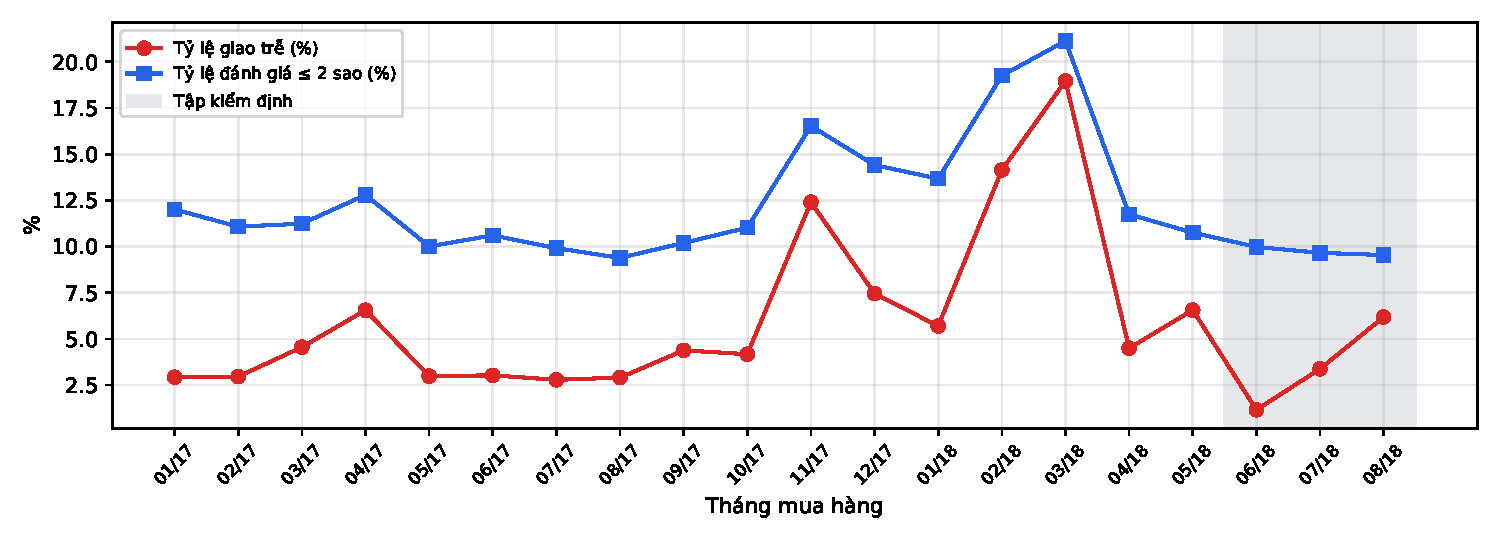
\includegraphics[width=0.95\textwidth]{Picture/monthly_late_review.pdf}
\caption{Tỷ lệ giao trễ và tỷ lệ đánh giá $\leq$ 2 sao theo tháng mua (vùng xám: tập kiểm định)}
\label{fig:monthly}
\end{figure}

\begin{table}[H]
\centering
\caption{Điểm đánh giá theo mức trễ so với ngày hẹn (đơn đã giao, có đánh giá)}
\label{tab:delay}
\begin{tabular}{@{}lrrr@{}}
\toprule
\textbf{Mức trễ} & \textbf{Số đơn} & \textbf{Điểm TB} & \textbf{Tỷ lệ $\leq$ 2 sao} \\
\midrule
Sớm $\geq$ 10 ngày & 61.528 & 4,32 & 8,9\% \\
Sớm 1--9 ngày & 26.640 & 4,23 & 9,9\% \\
Đúng ngày hẹn & 1.280 & 4,04 & 12,3\% \\
Trễ 1--3 ngày & 1.852 & 3,29 & 32,2\% \\
Trễ 4--7 ngày & 1.748 & 2,11 & 67,6\% \\
Trễ $>$ 7 ngày & 2.782 & 1,70 & 79,2\% \\
\bottomrule
\end{tabular}
\end{table}

\subsection{Kết quả hai mô hình DSS}
\label{sec:model-results}
\hspace{1cm}
Bảng~\ref{tab:metrics} tổng hợp chỉ số trên tập kiểm định 06--08/2018 (18.603 đơn cho mô hình
giao trễ, 18.520 đơn cho mô hình đánh giá thấp). PR-AUC cần được so với tỷ lệ nhãn dương (mức
của một mô hình đoán ngẫu nhiên).

\begin{table}[H]
\centering
\caption{Chỉ số đánh giá trên tập kiểm định 06--08/2018}
\label{tab:metrics}
\small\setlength{\tabcolsep}{4pt}
\begin{tabular}{@{}llrrrrrrr@{}}
\toprule
\textbf{Mô hình} & \textbf{Phiên bản} & \textbf{Dương} & \textbf{ROC-AUC} & \textbf{PR-AUC} &
\textbf{Ngưỡng} & \textbf{Prec.} & \textbf{Recall} & \textbf{F1} \\
\midrule
Giao trễ & HGB & 3,6\% & \textbf{0,868} & \textbf{0,519} & 0,5 & \textbf{0,750} & \textbf{0,415} & \textbf{0,534} \\
         & LogReg & 3,6\% & 0,837 & 0,268 & 0,5 & 0,449 & 0,144 & 0,219 \\
Đánh giá thấp & HGB & 9,7\% & \textbf{0,703} & \textbf{0,323} & 0,2 & \textbf{0,415} & \textbf{0,294} & \textbf{0,344} \\
              & LogReg & 9,7\% & 0,689 & 0,285 & 0,2 & 0,414 & 0,275 & 0,331 \\
\bottomrule
\end{tabular}
\end{table}

\begin{itemize}
    \item \textbf{Giao trễ}: PR-AUC 0,519 gấp khoảng 14 lần mức ngẫu nhiên (0,036) và gần gấp
          đôi baseline. Tại ngưỡng 0,5, cứ 4 đơn bị cảnh báo thì 3 đơn trễ thật, và phát hiện
          được 42\% số đơn trễ. Nếu Ops chỉ xử lý 10\% số đơn có điểm cao nhất thì phát hiện được
          63\% số đơn trễ.
    \item \textbf{Đánh giá thấp}: bài toán khó hơn vì điểm đánh giá còn phụ thuộc chất lượng sản
          phẩm, kỳ vọng của khách -- những yếu tố không có trong dữ liệu. PR-AUC 0,323 gấp 3,3 lần
          mức ngẫu nhiên; tại ngưỡng 0,2, 42\% khách được chọn đánh giá thấp thật, gấp 4,3 lần
          nếu chọn ngẫu nhiên.
\end{itemize}

Đường precision--recall (Hình~\ref{fig:pr}) nằm cao hơn hẳn mức ngẫu nhiên ở cả hai mô hình;
với mô hình giao trễ, precision gần 1 ở vùng recall dưới 0,2 (các đơn chắc chắn trễ).

\begin{figure}[H]
\centering
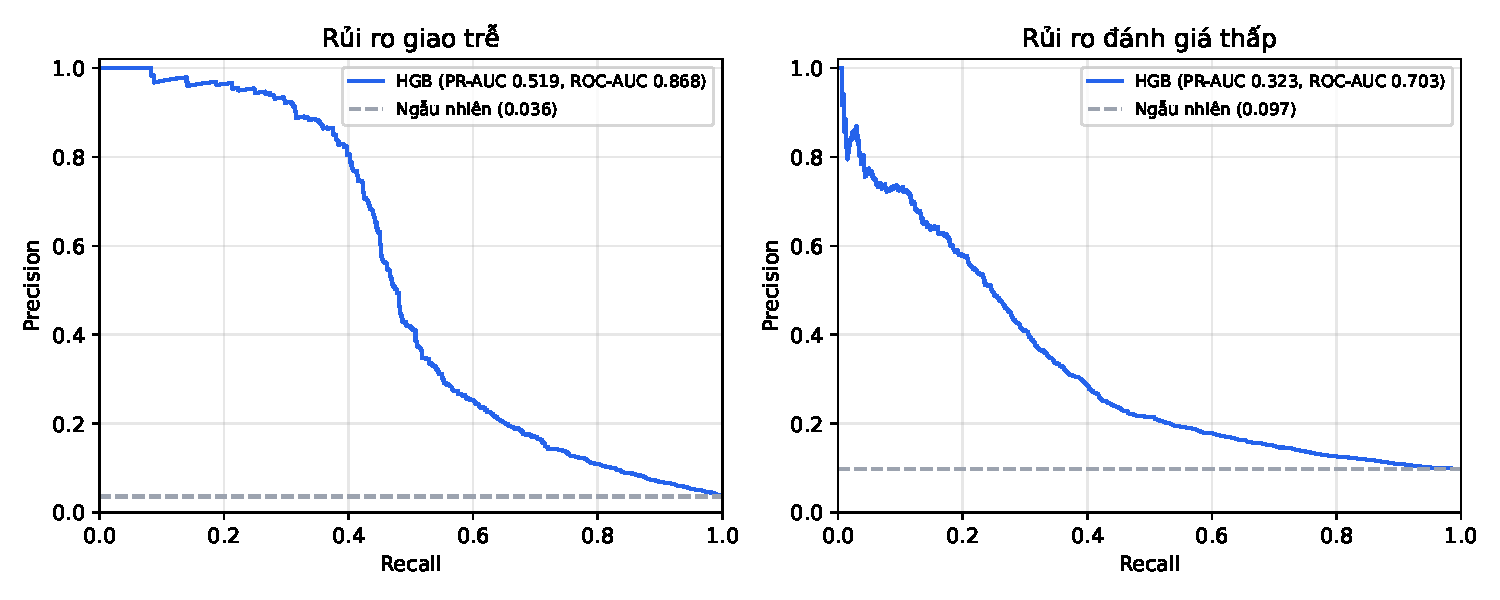
\includegraphics[width=0.95\textwidth]{Picture/pr_curves.pdf}
\caption{Đường precision--recall của mô hình HGB trên tập kiểm định}
\label{fig:pr}
\end{figure}

\textbf{Mức rủi ro có ý nghĩa thực tế} (Bảng~\ref{tab:levels}): tỷ lệ xảy ra thật giảm dần rõ
rệt từ High xuống Low, nên Ops có thể tin vào cách xếp mức để ưu tiên.

\begin{table}[H]
\centering
\caption{Số đơn và tỷ lệ xảy ra thật theo mức rủi ro (tập kiểm định)}
\label{tab:levels}
\begin{tabular}{@{}lrrrr@{}}
\toprule
& \multicolumn{2}{c}{\textbf{Giao trễ}} & \multicolumn{2}{c}{\textbf{Đánh giá thấp}} \\
\textbf{Mức} & \textbf{Số đơn} & \textbf{Trễ thật} & \textbf{Số đơn} & \textbf{$\leq$ 2 sao thật} \\
\midrule
High & 372 & 75,0\% & 1.276 & 41,5\% \\
Medium & 494 & 12,6\% & 2.443 & 12,6\% \\
Low & 17.737 & 1,9\% & 14.801 & 6,5\% \\
\bottomrule
\end{tabular}
\end{table}

\textbf{Đặc trưng quan trọng nhất} (permutation importance, mức giảm PR-AUC, Hình~\ref{fig:importance}):
\begin{itemize}
    \item Giao trễ: \texttt{slack\_days} (0,485) -- số ngày còn lại tới hạn sau khi bàn giao,
          \texttt{handoff\_vs\_\allowbreak limit\_days} (0,074) -- người bán bàn giao muộn so với hạn,
          bang của khách (0,010). Hàm ý: kiểm soát người bán bàn giao đúng hạn là đòn bẩy lớn
          nhất.
    \item Đánh giá thấp: \texttt{delay\_days} (0,127), số sản phẩm trong đơn \texttt{n\_items}
          (0,058), số người bán \texttt{n\_sellers} (0,011). Đơn nhiều sản phẩm/nhiều người
          bán dễ giao thiếu hoặc giao lệch nhau, dẫn tới đánh giá thấp.
\end{itemize}


\begin{figure}[H]
\centering
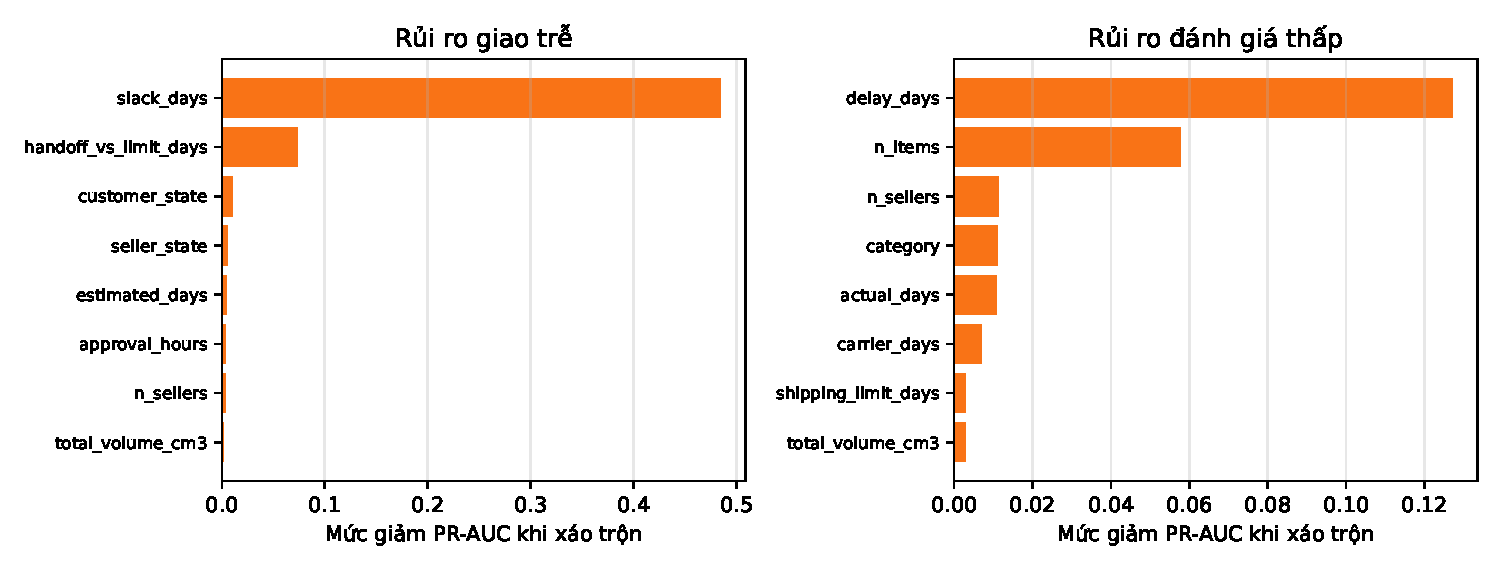
\includegraphics[width=0.95\textwidth]{Picture/feature_importance.pdf}
\caption{Permutation importance (top 8) của hai mô hình HGB}
\label{fig:importance}
\end{figure}

\subsection{Thí nghiệm bổ sung}
\begin{itemize}
    \item \textbf{Chấm điểm sớm hơn (ngay lúc đặt hàng)}: chỉ dùng các đặc trưng có lúc đặt
          hàng thì mô hình giao trễ đạt ROC-AUC 0,693, PR-AUC 0,073 (gần mức ngẫu nhiên); mô hình
          đánh giá thấp đạt ROC-AUC 0,620, PR-AUC 0,186. Điều này giải thích lựa chọn thời điểm
          chấm điểm ở Mục~5.2.
    \item \textbf{Chọn ngưỡng tối đa F1 trên validation}: với mô hình giao trễ, ngưỡng chọn được
          chỉ là 0,07 vì validation (03--05/2018) có tỷ lệ trễ cao bất thường (19\% ở 03/2018),
          áp sang tập kiểm định (3,6\%) cho F1 chỉ 0,207, so với 0,534 khi dùng ngưỡng theo chi
          phí. Với mô hình đánh giá thấp, hai cách cho kết quả gần nhau (0,323 so với 0,344).
          Đây là biểu hiện của \textit{data drift}: tỷ lệ nền thay đổi theo thời gian nên ngưỡng
          nên được đặt từ chi phí nghiệp vụ và được theo dõi định kỳ.
\end{itemize}

\subsection{Hạn chế}
\begin{itemize}
    \item Dataset dừng ở 10/2018 và là dữ liệu lịch sử tĩnh: các đơn ``đang vận chuyển''
          (1.106 đơn) thực chất là đơn bị kẹt trong dữ liệu gốc, nhiều đơn đã quá ngày hẹn.
    \item Không có dữ liệu về hãng vận chuyển, tuyến đường thực tế, thời tiết hay sự kiện (đình
          công, lễ hội) -- nguyên nhân của các đợt trễ tăng vọt -- nên mô hình không dự đoán
          được các cú sốc hệ thống.
    \item Mô hình đánh giá thấp chỉ đạt ROC-AUC 0,70: nội dung đánh giá (văn bản, 58--88\% bị
          trống), chất lượng sản phẩm thực tế không có trong dữ liệu có cấu trúc.
    \item Chi phí $C_{FP}$, $C_{FN}$ là giả định của nhóm, chưa được kiểm chứng bằng dữ liệu
          doanh nghiệp; ngưỡng thay đổi sẽ làm thay đổi precision/recall.
    \item Khoảng cách tính theo tọa độ trung bình của zip prefix và người bán đầu tiên của đơn
          (khoảng 1\% đơn có nhiều người bán).
    \item Công cụ dự đoán cho đơn tự nhập điền các đặc trưng thiếu bằng trung vị nên chỉ phản ánh
          một đơn ``điển hình''; mô hình học tương quan, không phải nhân quả, nên thay đổi các
          đại lượng hiếm gặp trong dữ liệu (như hạn bàn giao rất ngắn) có thể cho kết quả ngược
          trực giác.
    \item Olist là dữ liệu lịch sử nên chức năng gắn khách đang mô phỏng trên các đơn thuộc tập
          kiểm định (đã có review thật); hệ thống cũng chỉ lập danh sách, chưa gửi voucher hay gọi
          khách, nên chưa đo được hiệu quả chăm sóc thật.
\end{itemize}

\subsection{Thiếu sót của đề tài và định hướng mở rộng kho dữ liệu}
\label{sec:dw-gaps}
\hspace{1cm}
Khi đối soát hai bảng fact với các bảng chiều, nhóm nhận thấy nhiều thuộc tính được nạp vào
kho nhưng không có truy vấn nào sử dụng. Để thiết kế gọn và đúng phạm vi đề tài, các thuộc tính
này đã được \textbf{lược bỏ}; bảng chiều chỉ giữ những gì OLAP view, API và mô hình DSS đang
dùng, cùng các khóa tự nhiên cần cho ETL. Đây là một thiếu sót về độ phủ phân tích: kho dữ liệu
hiện trả lời tốt năm câu hỏi nghiệp vụ ở Mục~2.3 nhưng chưa hỗ trợ nhiều góc nhìn ad-hoc.
Bảng~\ref{tab:dropped-attrs} liệt kê các thuộc tính có thể bổ sung lại (dữ liệu nguồn vẫn còn
trong staging) và loại truy vấn ad-hoc mà chúng phục vụ trong tương lai.

\begin{table}[H]
\centering
\caption{Thuộc tính đã lược bỏ và truy vấn ad-hoc có thể phục vụ khi bổ sung lại}
\label{tab:dropped-attrs}
\small
\begin{tabular}{@{}>{\raggedright\arraybackslash}p{2.6cm}>{\raggedright\arraybackslash}p{4.6cm}>{\raggedright\arraybackslash}p{6.8cm}@{}}
\toprule
\textbf{Bảng chiều} & \textbf{Thuộc tính} & \textbf{Truy vấn ad-hoc trong tương lai} \\
\midrule
\texttt{DIM\_DATE} & quý, mùa (Nam bán cầu), cuối tuần, tuần trong năm, tên thứ/tháng &
Phân tích mùa vụ (doanh thu, tỷ lệ trễ theo quý/mùa), so sánh đơn đặt cuối tuần và ngày thường,
báo cáo theo tuần. \\
\texttt{DIM\_PRODUCT} & tên ngành gốc, độ dài tên/mô tả, số ảnh, khối lượng, thể tích &
Chất lượng trang sản phẩm (số ảnh, độ dài mô tả) so với điểm đánh giá; sản phẩm nặng/cồng kềnh
có dễ giao trễ không. \\
\texttt{DIM\_SELLER} & zip, thành phố, vùng & Hiệu suất giao hàng theo vùng hoặc thành phố
của người bán, tuyến vùng $\to$ vùng. \\
\texttt{DIM\_LOCATION} & tên bang, quốc gia & Hiển thị báo cáo bằng tên đầy đủ, mở rộng sang
thị trường ngoài Brazil. \\
\texttt{DIM\_CUSTOMER} & ngày mua đầu tiên & Phân tích cohort, so sánh khách mới và khách quay
lại. \\
\bottomrule
\end{tabular}
\end{table}

Ngược lại, một số \textbf{khóa ngoại} chưa được truy vấn nào dùng nhưng vẫn được \textbf{giữ lại}
vì chúng là khung của star schema và chi phí lưu trữ thấp:
\texttt{customer\_sk}, \texttt{seller\_sk}, \texttt{payment\_type\_sk} trong
\texttt{FACT\_ORDER\_ITEM} (phân tích doanh thu theo khách, người bán, phương thức thanh toán),
và bốn vai trò ngày \texttt{approved\_date\_sk}, \texttt{carrier\_date\_sk},
\texttt{delivered\_date\_sk}, \texttt{estimated\_date\_sk} trong
\texttt{FACT\_ORDER\_FULFILLMENT} (thống kê theo tháng giao hàng hoặc tháng bàn giao thay vì
tháng mua). Định hướng mở rộng:
\begin{itemize}
    \item Bổ sung lại các thuộc tính trong Bảng~\ref{tab:dropped-attrs} khi có câu hỏi nghiệp vụ
          cụ thể, kèm OLAP view và bộ lọc tương ứng trên Manager Dashboard (ví dụ bộ lọc quý,
          mùa).
    \item Xây thêm OLAP view theo các vai trò ngày khác của \texttt{FACT\_ORDER\_FULFILLMENT}
          và theo người bán, khách hàng của \texttt{FACT\_ORDER\_ITEM}.
    \item Duy trì bước đối soát fact -- dimension (khóa NULL, dòng chiều không được tham chiếu,
          thuộc tính không được dùng) như một phần của kiểm tra chất lượng định kỳ; chính bước
          này đã giúp phát hiện lỗi mốc hiệu lực SCD2 theo ngày (Mục~3.2).
\end{itemize}

\subsection{Hướng phát triển}
\begin{itemize}
    \item Chấm điểm lại nhiều lần trong vòng đời đơn (lúc duyệt, lúc bàn giao, mỗi ngày khi đang
          vận chuyển) thay vì một thời điểm cố định.
    \item Thêm đặc trưng lịch sử vận hành (tỷ lệ trễ gần đây theo tuyến, theo người bán) tính
          theo cửa sổ thời gian, kèm cơ chế giám sát drift và tự huấn luyện lại.
    \item Hiệu chỉnh xác suất (\textit{calibration}) và cho phép Ops nhập chi phí trên giao diện
          để tự điều chỉnh ngưỡng.
    \item Đo hiệu quả thật của chiến dịch chăm sóc bằng thử nghiệm A/B (nhóm được tặng voucher và
          nhóm đối chứng) để ước lượng lại $C_{FN}$.
    \item Khai thác nội dung đánh giá (xử lý ngôn ngữ tự nhiên tiếng Bồ Đào Nha) để hiểu nguyên
          nhân đánh giá thấp.
\end{itemize}
